% Generated from content.json by scripts/render_cv.py.
% Edit the shared content or this layout template, then run scripts/build.py.
% Compile from cv/: xelatex -interaction=nonstopmode -halt-on-error <filename>.tex
% Requires XeLaTeX, fontspec, and (for Chinese) xeCJK plus Noto Sans SC / CJK SC
% or the Fandol fonts supplied by a standard TeX Live Chinese installation.
\documentclass[10pt,a4paper]{article}
\usepackage[a4paper,top=0.8cm,bottom=0.8cm,left=1.55cm,right=1.55cm]{geometry}
\usepackage{fontspec}

\usepackage{graphicx}
\usepackage{tabularx}
\usepackage{array}
\usepackage{enumitem}
\usepackage{titlesec}
\usepackage{xcolor}
\usepackage{hyperref}
\usepackage{microtype}

\defaultfontfeatures{Ligatures=TeX}
\IfFontExistsTF{TeX Gyre Heros}
  {\setmainfont{TeX Gyre Heros}}
  {\IfFontExistsTF{Arimo}
    {\setmainfont{Arimo}}
    {\setmainfont{Latin Modern Sans}}}

\definecolor{navy}{HTML}{163A5F}
\definecolor{slate}{HTML}{4B5563}
\definecolor{rulegray}{HTML}{C9D1D9}
\hypersetup{
  colorlinks=true,
  urlcolor=navy,
  linkcolor=navy,
  pdfauthor={Shiyu Shen},
  pdftitle={Shiyu Shen -- Academic Curriculum Vitae}
}
\urlstyle{same}
\pagestyle{empty}
\setlength{\parindent}{0pt}
\setlength{\parskip}{0pt}
\setlength{\tabcolsep}{0pt}
\setlist[itemize]{leftmargin=1.25em,itemsep=0.5pt,topsep=1pt,parsep=0pt,partopsep=0pt}
\setlist[enumerate]{leftmargin=1.55em,itemsep=2pt,topsep=3pt,parsep=0pt,partopsep=0pt}
\titleformat{\section}
  {\large\bfseries\color{navy}}
  {}{0pt}{}
  [\vspace{1pt}\color{rulegray}\titlerule]
\titlespacing*{\section}{0pt}{5pt}{3pt}

\newcommand{\cvrow}[3]{%
  \begin{tabularx}{\textwidth}{@{}>{\raggedright\arraybackslash}p{3.30cm}X>{\raggedleft\arraybackslash}p{2.20cm}@{}}
    \mbox{\textbf{#1}} & {\hyphenpenalty=10000\exhyphenpenalty=10000 #2} &
    \textcolor{slate}{\mbox{#3}}
  \end{tabularx}\vspace{2pt}
}
\newcommand{\projectline}[3]{%
  \begin{tabularx}{\textwidth}{@{}X>{\raggedleft\arraybackslash}p{2.25cm}@{}}
    \small\textbf{#1}\if\relax\detokenize{#2}\relax\else\textbf{:} #2\fi &
    \small\textcolor{slate}{\mbox{#3}}
  \end{tabularx}\vspace{0.5pt}
}
\newcommand{\me}{\textbf{Shiyu Shen}}
\newcommand{\status}[1]{\textcolor{slate}{\textit{#1}}}
% The inner explicit color also keeps titles black when urlcolor is changed.
\newcommand{\papertitle}[2]{\href{#1}{\textcolor{black}{#2}}}

\newcommand{\contactblock}{%
  {\fontsize{25}{29}\selectfont\bfseries\color{navy} Shiyu Shen}\\[3pt]
  Nankai University, Tianjin, China\\[3pt]
  \href{mailto:shenshiyu@mail.nankai.edu.cn}{shenshiyu@mail.nankai.edu.cn}
  \enspace\textcolor{rulegray}{|}\enspace
  (+86) 151 2233 9659\\[3pt]
  \url{https://github.com/Teemo341}\\[3pt]
  \url{https://scholar.google.com/citations?user=rNZgWagAAAAJ\&hl=en}
}
\begin{document}
\thispagestyle{empty}
\IfFileExists{../assets/portrait.jpg}{%
  \begin{minipage}[c]{0.17\textwidth}
    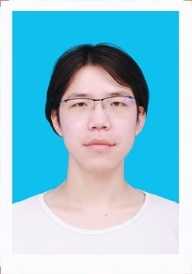
\includegraphics[width=2.20cm,height=2.95cm,keepaspectratio]{../assets/portrait.jpg}
  \end{minipage}%
  \hfill
  \begin{minipage}[c]{0.80\textwidth}
    \contactblock
  \end{minipage}
}{\contactblock}

\section{Research Profile}
\begin{itemize}
  \item My research focuses on uncertainty in machine learning, Bayesian deep learning, and domain generalization.
  \item In-depth understanding of the foundations of diffusion/flow models and LLMs.
  \item Proficient in PyTorch, verl, and slime, with hands-on experience in large-scale pretraining, SFT and RL.
  \item Extensive project experience spanning model development, system integration, and deployment.
\end{itemize}
\section{Education}
\cvrow{Nankai University}{Bachelor’s degree; Gongneng Scholarship}{2017–2021}
\cvrow{Nankai University}{Master’s degree; Gongneng Scholarship, Zhou Enlai Scholarship, National Scholarship}{2021–2024}
\cvrow{Nankai University}{Ph.D. studies; National Scholarship}{2024–2028}
\section{Publications \& Preprints}
\begin{enumerate}
  \item Z. Wang, B. Pan, \me, T. Shi, and Z. Shi. ``\papertitle{https://arxiv.org/abs/2406.05628}{Domain Generalization Guided by Large-Scale Pre-Trained Priors.}'' \textit{arXiv preprint arXiv:2406.05628}, 2024.
  \item Y. Tan, J. Wu, Y. Liu, \me, X. Xu, and B. Pan. ``\papertitle{https://doi.org/10.3390/rs16234545}{A Lightweight Transformer-Based Spatiotemporal Analysis Prediction Algorithm for High-Dimensional Meteorological Data.}'' \textit{Remote Sensing}, 2024.
  \item \me, B. Pan, Y. Wang, Y. Liu, and Z. Shi. ``\papertitle{https://ieeexplore.ieee.org/document/10852282}{A Second Order Stationarity Based Confidence Assessment Method for Temperature Forecast.}'' \textit{IEEE Geoscience and Remote Sensing Letters}, 2025.
  \item \me, B. Pan, Z. Zhang, and Z. Shi. ``\papertitle{https://arxiv.org/abs/2506.02601}{Hyperspectral Image Generation with Unmixing Guided Diffusion Model.}'' \textit{arXiv preprint arXiv:2506.02601}, 2025. \status{Under review at IEEE TGRS.}
  \item \me, B. Pan, and G. Xue. ``\papertitle{https://arxiv.org/abs/2506.02654}{A Pretrained Probabilistic Transformer for City-Scale Traffic Volume Prediction.}'' \textit{arXiv preprint arXiv:2506.02654}, 2025. \status{Under review at IEEE TMM.}
  \item \me, Z. Gao, T. Chai, Y. Huang, and B. Pan. ``\papertitle{https://arxiv.org/abs/2511.22958}{Contrastive Heliophysical Image Pretraining for Solar Dynamics Observatory Records.}'' \textit{arXiv preprint arXiv:2511.22958}, 2025.
  \item Z. Gao, \me, X. Xiang, W. Li, Y. Gao, and Q. Fan. ``\papertitle{https://openreview.net/forum?id=08pxmTLKTT}{SmartSAM: Segment Ambiguous Objects like Smart Annotators.}'' 2025.
  \item \me, B. Pan, T. Shi, T. Li, and Z. Shi. ``\papertitle{https://doi.org/10.1016/j.patcog.2026.113084}{Be Bayesian by Attachments to Catch More Uncertainty.}'' \textit{Pattern Recognition}, 2026.
  \item B. Pan, \me, Z. Wang, Z. Shi, and X. Xu. ``\papertitle{https://arxiv.org/abs/2508.16976}{Preserving Domain Generalization in Fine-Tuning via Joint Parameter Selection.}'' \textit{IEEE Transactions on Multimedia}, 2026.
  \item Z. Gao, \me, T. Chai, W. Wang, H. Xu, W. Li, et al. ``\papertitle{https://arxiv.org/abs/2603.25021}{VideoTIR: Accurate Understanding for Long Videos with Efficient Tool-Integrated Reasoning.}'' \textit{European Conference on Computer Vision (ECCV)}, 2026.
  \item \me, B. Pan, T. Shi, T. Li, and Z. Shi. ``\papertitle{https://arxiv.org/abs/2310.16277}{Bayesian Domain Invariant Learning via Posterior Generalization of Parameter Distributions.}'' \textit{arXiv preprint arXiv:2310.16277}, 2026. \status{Under review at Pattern Recognition.}
  \item \me, B. Pan, Z. Wang, and Z. Shi. ``\papertitle{https://scholar.google.com/scholar?q=\%22A\%20Distribution-Free\%20Efficient\%20Bayesian\%20Framework\%20for\%20Domain\%20Generalization\%22}{A Distribution-Free Efficient Bayesian Framework for Domain Generalization.}'' 2026. \status{Under review at IEEE TMM.}
\end{enumerate}
\section{Research \& Engineering Projects}
\projectline{UAV Electro-Optical Imaging Teaching System}{Scene-generation subsystem.}{2024}
\projectline{Maritime Optical Data Analysis System}{Confidence-assessment subsystem.}{2024}
\projectline{Inertial Navigation High-Order Error Identification}{Project lead; big-data regression analysis.}{2025}
\projectline{Virtual–Real Intelligent Traffic Simulation Platform}{Traffic-volume prediction and signal control.}{2025}
\section{Research \& Industry Experience}
\projectline{Tianrang — TRFold}{}{2021}
\projectline{Yunqi Engineering Institute — Intelligent Transportation}{Train traffic prediction and signal-control models.}{2024}
\projectline{Zhejiang Lab — AstrOne}{Lead SolarCLIP and SolarGPT development.}{2024}
\projectline{Zhejiang Lab — 021 Chemical LLM}{Lead SFT and GRPO; design curriculum learning.}{2025}
\projectline{Zhejiang Lab — 021 Mathematics LLM}{Build CPT data.}{2025}
\projectline{Zhejiang Lab — 021 Code Agent}{Design stepwise verifiable RL rewards.}{2026–Present}
\end{document}
